\section{Introduction}
\label{sec:introduction}

The Transmission Control Protocol, short TCP, is most popular communication
protocol on the Internet. To make it scalable and adaptive to the current
condition of network without overloading it, congestion control mechanism are
used. Part of these algorithm is TCP slow start as described in
RFC5681~\cite{rfc5681}.

The TCP slow algorithm limits the number of bytes it sends on a new TCP
connection before waiting for an acknowledgement. On every acknowledged packet
the sender increases the window size by one segment until the Slow-start
threshold (\emph{ssthres}) is reached  or the receiver advertises a lower
receiver window (\emph{rwnd}) in its TCP header. The exponential grow of the
window every roundtrip will be also stopped if TCP detects packet loss. This
could be indicated by either a duplicate acknowledgement of the receiver or a
timeout. Depending on the congestion algorithm in use the sender will then
behave differently. TCP Reno~\cite{rfc2581} is currently the most widely
deployed. On timeout it will reduce the congestion window to 1. If it receives
an acknowledgement for the same packet three times in a row, it will half
congestion window. The new Slow-Start threshold will be set to the current
window. The sender assumes that the packet after the one, it received duplicate
ACKs for, got lost and will perform a retransmit (also known as Fast
Retransmit). It then enters a phase called Fast Recovery. In this phase the
sender will increase the congestion window only one segment per round trip,
which is equivalent to linear growth.

Other congestion algorithm have slightly different behaviour on how they behave
when congestion is detected. In picture~\ref{fig:cwnd_tcp_algos} the grow of TCP
congestion windows for different TCP congestion algorithm is depicted. An
Assumption most algorithms make is that the majority packet loss in the network
occurs because overloading the network at bottlenecks rather than faulty
transmission. Routers in the network have a limited queue they fill up, before
they begin to drop IP packets. Bottlenecks in the network occur because
connected links have asymmetric bandwidth or usage.

\begin{figure*}[ht]
\footnotesize
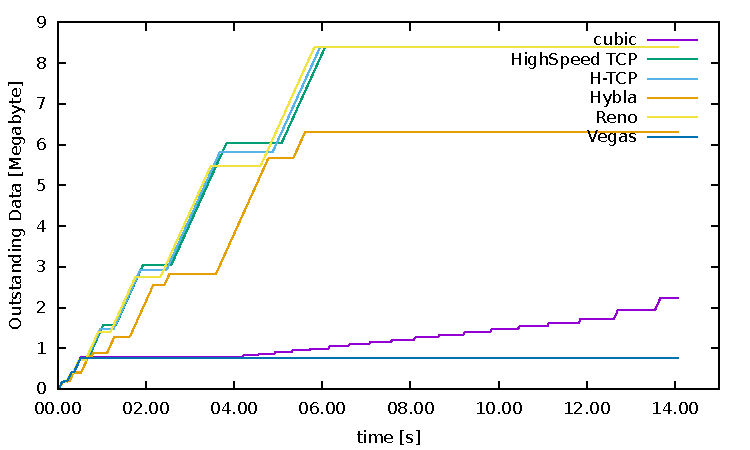
\includegraphics[scale=1]{figure/b2a_owin.pdf}
\caption{Congestion window grow over time for different TCP congestion
algorithm for a single connection over 10mbit link with a forwarding delay of
10ms when downloading 16MiB file over HTTP}
\label{fig:cwnd_tcp_algos}
\end{figure*}

The task of a TCP congestion algorithms is to manage this network resources by
scaling the window of outstanding bytes accordingly. This has a direct effect on
throughput. The actual bandwidth of TCP connection is calculated in the
following way~\cite{opac-b1120676}:

\begin{align}
  Throughput &= \frac{cwnd * MTU}{RTT} \\
  MTU~&\dots~\text{Maximum Transfer Unit [bytes]} \nonumber\\
  cwnd~&\dots~\text{Outstanding segments} \nonumber\\
  RTT~&\dots~\text{Round trip time between} \nonumber\\
      &~~~~\text{sender and receiver [s]} \nonumber\\
  Throughput~&\dots~\text{bandwidth of the sender [bytes/s]} \nonumber
\end{align}

The initial congestion window therefor is a critical factor at the start of a
new connection. If it is chosen too high their is a risk of overloading the
network which results in dropped packets followed by retransmission. If it is
too low a connection will take longer to fully use the available bandwidth on the
link. This is especially important if only small payloads are transmitted. For
these connections it might happen that the data is transferred before the full
congestion window could be build up.

One of the most important applications of the TCP these days is the web. A
common web page consists of multiple resources like HTML-Code, CSS style-sheets
and pictures. To load such a page a browser has to issue multiple HTTP-Requests.
According to httparchive.org\cite{httparchive}, which collect statistical data
of the top million pages of the web, reports that on average 101 requests are
required to serve to serve a single page\cite{httparchive-trends}. The amount of
data per request add up to \emph{22,4kB} excluding the overhead of TCP itself.
The browser opens 40 TCP Connections on average. The number of requests is
higher than for the number of connections, which means for some requests
existing connections could be reused, by using for example HTTP
Keep-Alive~\cite{I-D.thomson-hybi-http-timeout}.

Having this many requests increases the page load time and lead to a certain
latency before a web page can be rendered completely. The time to complete a
transfer using TCP slow start assuming no packets get lost is calculated the
follow way~\cite{832574}:

\begin{align}
  t&=\lceil log_{\gamma} (\frac{S(\gamma - 1)}{init\_cwnd} + 1) \rceil * RTT +
  \frac{S}{C} \label{loadtime}\\\label{transfer_time}
  S~&\dots~\text{transfer size } \\\nonumber
  init\_cwnd~&\dots~\text{Initial window size} \\\nonumber
  RTT~&\dots~\text{Round-Trip-Time} \\\nonumber
  C~&\dots~\text{Link Rate of the slowest link} \\\nonumber
\end{align}
\begin{align}
  & && \text{delayed ACKs} \nonumber \\
  \gamma &=
    \smash{\left\{\begin{array}{lr}
       1.5 \\[\jot]
       2 \\\nonumber
       \vspace{0.5em}
   \end{array}\right.} && \text{not delayed} \\\nonumber
\end{align}

A report by google called \emph{More Bandwidth Doesn't Matter}\cite{bandwith}
indicates that browsers cannot make effective use of broadband connections to
speed up page load time. The study shown that an increase of bandwidth from
5Mbps to 10Mbps only gave 5\% improvement in load time. On the other hand
changing the Round Trip time had much higher impact: With a high RTT (220ms)
only 10\% of 5Mbps connection could be used, while an almost zero Round trip
time (still only) allowed to use 54\% of the bandwidth.

To reduce the time most browsers issue 6 to 13 parallel requests per
domain~\cite{browserscope}. Website master can increase these parallelism
further by using multiple domains for resources. While this approach improves
load time it pretty inefficient, because every TCP connection has to build its
own congestion window. Also these connection compete with each other for
bandwidth and circumvent TCP congestion avoidance.

A better alternative to multiple connection to improve the load time might be to
increase the initial congestion window as we see in equation \ref{loadtime}. The
current standard rfc3390 from 2002 proposes a windows size of 2 to 4 segments.
In praxis often a window of 3 was chosen, which correspond to the size of an
Ethernet Frame (4kb). However since then the bandwidth has been dramatically
increased: According to Akamai's report \emph{State of the
internet}~\cite{q3-2015-soti-connectivity-final} the global average bandwidth is
now 5.1Mbps.

So there is an growing demands for an adaption of the initial window size. In
2009 Google published the result of an internal large scale
experiment~\cite{36640}. From measurements over 2 weeks they experienced on
average an latency improvement of 10\%, when using a window of 10 segments. On
the hand the retransmission rate due more lost package only rise up 0.5\%. On
networks with a high bandwidth delay product (where either the RTT, the
bandwidth or both is high) and on networks with higher RTT, the acceleration was
even higher. This is to be expected because more packets can be transmitted
before an acknowledgement has to reach back the sender. Their reasoning for the
improvement was that 90\% of all requests of the top 500 webpages actually fit
within the first 10 segments.

Also short bursty HTTP Requests have to compete with longer flows such as
video streams or downloads. This effect is also known as "elephant
flow"~\cite{992898}. Because continous tcp connection will have the maximum
possible congestion window, they will get a disproportionate share of the total
bandwidth in contrast the shorter connection.

As result of these experiments IETF released in 2010 an Internet
Draft~\cite{draft-ietf-tcpm-initcwnd-00} to increase the initial window by the
same amount, which became an experimental standard in 2013
(rfc6928~\cite{rfc6928}). The Linux operating system also early on adapt to this
scheme in 2011~\cite{linux}. Almost all Content Delivery Networks these days
have at least an initial window of 10 as baseline set~\cite{cdnplanet}. Some of
them go even further and have a higher window such as Cachefly, which sends a
burst of 70 packets.
